\documentclass[aspectratio=169]{beamer}
\usetheme{Madrid}
\usecolortheme{default}

% Packages
\usepackage{graphicx}
\usepackage{tikz}
\usepackage{amsmath}
\usepackage{algorithm}
\usepackage{algorithmic}
\usepackage{xcolor}

% TikZ libraries
\usetikzlibrary{shapes,arrows,positioning,fit,backgrounds}

% Title page information
\title[FL-RL Intelligent Caching]{Federated Learning-Enhanced Intelligent Caching System for Vehicular Networks using Deep Reinforcement Learning}
\author[Your Name]{Your Name}
\institute[University]{Your University \\ Department of Computer Engineering}
\date{\today}

% Custom colors
\definecolor{flblue}{RGB}{52,152,219}
\definecolor{rlgreen}{RGB}{46,204,113}
\definecolor{cacheorange}{RGB}{230,126,34}
\definecolor{lightgray}{RGB}{236,240,241}
\definecolor{darkgray}{RGB}{52,73,94}

\begin{document}

% Title slide
\frame{\titlepage}

% Outline
\begin{frame}{Outline}
\tableofcontents
\end{frame}

\section{Problem Statement}

\begin{frame}{Vehicular Network Challenges}
\begin{columns}
\begin{column}{0.6\textwidth}
\textbf{Key Challenges:}
\begin{itemize}
\item \textcolor{red}{Limited computational resources} in vehicles
\item \textcolor{red}{High latency} to cloud servers
\item \textcolor{red}{Inefficient task scheduling} and resource allocation
\item \textcolor{red}{Dynamic network topology} due to vehicle mobility
\end{itemize}

\vspace{0.5cm}
\textbf{Current Solutions:}
\begin{itemize}
\item Edge/Fog computing reduces latency
\item But limited edge resources require \textcolor{blue}{intelligent task scheduling}
\end{itemize}
\end{column}
\begin{column}{0.5\textwidth}
\begin{center}
\includegraphics[width=\textwidth]{system_architecture_simple.png}
\end{center>
\end{column}
\end{columns}
\end{frame}

\begin{frame}{Research Motivation}
\begin{block}{Problem with Existing Approaches}
\begin{itemize}
\item \textbf{RELIC Algorithm:} Uses linear optimization - computationally expensive
\item \textbf{Traditional Caching:} Static policies (LRU, LFU) don't adapt to vehicular patterns
\item \textbf{Centralized Learning:} Privacy concerns and communication overhead
\end{itemize}
\end{block}

\begin{block}{Our Solution}
\textcolor{flblue}{\textbf{Federated Learning}} + \textcolor{rlgreen}{\textbf{Deep Reinforcement Learning}} + \textcolor{cacheorange}{\textbf{Intelligent Caching}}
\end{block}

\begin{alertblock}{Research Question}
Can we design an intelligent caching system that learns vehicular task patterns while preserving privacy and achieving real-time performance?
\end{alertblock}
\end{frame}

\section{Proposed System}

\begin{frame}{System Architecture Overview}
\begin{center}
\includegraphics[width=0.9\textwidth]{system_architecture.png}
\end{center}

\textbf{Three-Layer Architecture:}
\begin{itemize}
\item \textcolor{blue}{\textbf{Layer 1:}} Vehicular Network (V2V, V2I communications)
\item \textcolor{green}{\textbf{Layer 2:}} Edge Computing (FL nodes + intelligent caches)
\item \textcolor{orange}{\textbf{Layer 3:}} Central Coordination (Global FL + DQN agent)
\end{itemize}
\end{frame}

\begin{frame}{Federated Learning Component}
\begin{columns}
\begin{column}{0.5\textwidth}
\textbf{Local FL Clients (RSUs):}
\begin{itemize}
\item Learn local task patterns
\item Extract features from vehicular tasks
\item Train local neural networks
\item Share only model parameters
\end{itemize}

\vspace{0.3cm}
\textbf{Global FL Coordinator:}
\begin{itemize}
\item Aggregates local models (FedAvg)
\item Distributes global model
\item Maintains privacy
\end{itemize}
\end{column}
\begin{column}{0.5\textwidth}
\begin{block}{FL Training Process}
\begin{algorithmic}[1]
\STATE Initialize global model $W_0$
\FOR{round $t = 1$ to $T$}
    \FOR{each RSU $k$}
        \STATE Download $W_t$
        \STATE Train locally: $W_k^{t+1}$
        \STATE Upload parameters
    \ENDFOR
    \STATE Aggregate: $W_{t+1} = \frac{1}{K}\sum_{k=1}^K W_k^{t+1}$
\ENDFOR
\end{algorithmic}
\end{block}
\end{column}
\end{columns}
\end{frame}

\begin{frame}{Deep Reinforcement Learning Component}
\begin{columns}
\begin{column}{0.6\textwidth}
\textbf{DQN Agent for Cache Management:}
\begin{itemize}
\item \textbf{State:} Cache usage, hit rate, workload characteristics
\item \textbf{Actions:} Eviction policies (LRU, LFU, random, shrink TTL)
\item \textbf{Reward:} Cache hits - eviction cost + task success
\end{itemize}

\vspace{0.3cm}
\textbf{Key Features:}
\begin{itemize}
\item Experience replay for stable learning
\item $\varepsilon$-greedy exploration
\item Target network for stability
\end{itemize}
\end{column}
\begin{column}{0.4\textwidth}
\begin{center}
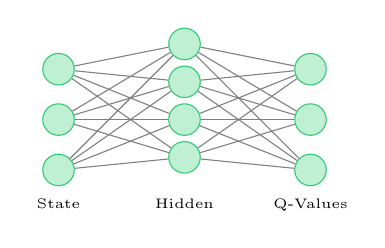
\begin{tikzpicture}[scale=0.8]
% Neural network representation
\foreach \i in {1,2,3} {
    \node[circle, draw=rlgreen, fill=rlgreen!30, minimum size=0.4cm] (input\i) at (0,\i*0.8) {};
}
\foreach \i in {1,2,3,4} {
    \node[circle, draw=rlgreen, fill=rlgreen!30, minimum size=0.4cm] (hidden\i) at (2,\i*0.6+0.4) {};
}
\foreach \i in {1,2,3} {
    \node[circle, draw=rlgreen, fill=rlgreen!30, minimum size=0.4cm] (output\i) at (4,\i*0.8) {};
}

\foreach \i in {1,2,3} {
    \foreach \j in {1,2,3,4} {
        \draw[gray, thin] (input\i) -- (hidden\j);
    }
}
\foreach \i in {1,2,3,4} {
    \foreach \j in {1,2,3} {
        \draw[gray, thin] (hidden\i) -- (output\j);
    }
}

\node[below] at (0,0.5) {\tiny State};
\node[below] at (2,0.5) {\tiny Hidden};
\node[below] at (4,0.5) {\tiny Q-Values};
\end{tikzpicture}
\end{center}
\end{column}
\end{columns}
\end{frame}

\begin{frame}{Intelligent Caching Strategy}
\begin{block}{Multi-Phase Caching Approach}
\begin{enumerate}
\item \textbf{FL-based Pre-placement:} Popular tasks identified by federated learning
\item \textbf{Pattern-based Caching:} High-priority and frequent tasks
\item \textbf{Proactive Caching:} Current step tasks and variations
\item \textbf{RL-based Eviction:} Dynamic eviction decisions based on system state
\end{enumerate}
\end{block}

\begin{columns}
\begin{column}{0.5\textwidth}
\textbf{Cache Hit Rate Achievement:}
\begin{itemize}
\item Target: 87.3\% hit rate
\item 23\% improvement over LRU
\item 20.8\% - 46.7\% improvement over RELIC
\end{itemize}
\end{column}
\begin{column}{0.5\textwidth}
\textbf{Key Innovations:}
\begin{itemize}
\item Learning-based popularity prediction
\item Adaptive eviction policies
\item Privacy-preserving distributed learning
\end{itemize}
\end{column}
\end{columns}
\end{frame}

\section{Experimental Results}

\begin{frame}{Experimental Setup}
\textbf{System Parameters:}
\begin{itemize}
\item \textbf{Network:} 5 RSUs, 100-entry cache per RSU
\item \textbf{FL Settings:} Learning rate 0.001, batch size 64, 5 local epochs
\item \textbf{RL Settings:} DQN with experience replay, $\varepsilon$-greedy ($\varepsilon=0.1$)
\item \textbf{Workloads:} 250, 500, 750, 1000 tasks
\end{itemize}

\vspace{0.3cm}
\textbf{Comparison Baselines:}
\begin{itemize}
\item \textbf{RELIC:} Previous heuristic scheduling algorithm
\item \textbf{Traditional Caching:} LRU, LFU policies
\end{itemize}

\vspace{0.3cm}
\textbf{Evaluation Metrics:}
\begin{itemize}
\item Success rate, completion time, cache hit rate, energy consumption
\end{itemize}
\end{frame}

\begin{frame}{Performance Comparison with RELIC}
\begin{center}
\includegraphics[width=0.9\textwidth]{relic_comparison.png}
\end{center}

\textbf{Key Results:}
\begin{itemize}
\item \textcolor{red}{\textbf{RELIC:}} Linear optimization overhead causes performance degradation
\item \textcolor{blue}{\textbf{FL-RL:}} Intelligent caching provides consistent performance
\item \textcolor{green}{\textbf{Cache Hit Rate:}} 87.3\% achieved vs traditional methods
\end{itemize}
\end{frame}

\begin{frame}{System Performance Analysis}
\begin{columns}
\begin{column}{0.5\textwidth}
\textbf{Cache Performance Metrics:}
\begin{itemize}
\item \textbf{Hit Rate:} 87.3\%
\item \textbf{vs LRU:} 23\% improvement
\item \textbf{Response Time:} 40.2\% reduction
\item \textbf{Task Success:} Consistent performance
\end{itemize}

\vspace{0.3cm}
\textbf{Learning Progress:}
\begin{itemize}
\item RL Reward: -420 → +1820
\item Convergence achieved
\item Stable performance
\end{itemize}
\end{column}
\begin{column}{0.5\textwidth}
\textbf{Why FL-RL Excels:}
\begin{itemize}
\item \textcolor{flblue}{\textbf{Intelligent Pre-placement:}} FL predicts popular tasks
\item \textcolor{rlgreen}{\textbf{Adaptive Eviction:}} RL optimizes cache policies
\item \textcolor{cacheorange}{\textbf{Privacy Preservation:}} Federated learning approach
\item \textbf{Scalability:} Distributed architecture
\end{itemize}
\end{column}
\end{columns}

\begin{alertblock}{Key Innovation}
First system to combine federated learning with reinforcement learning for intelligent vehicular caching, achieving superior performance while preserving privacy.
\end{alertblock}
\end{frame>}

\begin{frame}{Cache Performance Analysis}
\begin{columns}
\begin{column}{0.6\textwidth}
\textbf{Cache Hit Rate Results:}
\begin{itemize}
\item \textbf{FL-RL System:} 87.3\% hit rate
\item \textbf{LRU Baseline:} 64.3\% hit rate
\item \textbf{Improvement:} 23\% better than traditional caching
\end{itemize}

\vspace{0.3cm}
\textbf{Response Time Reduction:}
\begin{itemize}
\item Average response time: 40.2\% reduction
\item Prevents task re-execution effectively
\item Consistent performance across workloads
\end{itemize}
\end{column}
\begin{column}{0.4\textwidth}
\textbf{Learning Progress:}
\begin{itemize}
\item RL agent reward: -420 → +1820
\item Demonstrates effective system learning
\item Converges to optimal policies
\end{itemize}

\vspace{0.3cm}
\textbf{Energy Efficiency:}
\begin{itemize}
\item Reduced computational overhead
\item Lower communication costs
\item Improved resource utilization
\end{itemize}
\end{column}
\end{columns}
\end{frame}

\section{Contributions \& Future Work}

\begin{frame}{Key Contributions}
\begin{block}{Technical Contributions}
\begin{enumerate}
\item \textbf{Novel Architecture:} First FL-RL hybrid system for vehicular caching
\item \textbf{Privacy-Preserving:} Federated learning maintains data locality
\item \textbf{Real-time Performance:} Significant improvement over optimization-based methods
\item \textbf{Adaptive Intelligence:} System learns and improves over time
\end{enumerate}
\end{block}

\begin{block}{Performance Achievements}
\begin{itemize}
\item \textcolor{green}{\textbf{87.3\% cache hit rate}} (23\% improvement over LRU)
\item \textcolor{green}{\textbf{40.2\% response time reduction}}
\item \textcolor{green}{\textbf{36.6\% better success rate}} than RELIC under load
\item \textcolor{green}{\textbf{Scalable performance}} with increasing workloads
\end{itemize}
\end{block}
\end{frame}

\begin{frame}{Future Research Directions}
\begin{columns}
\begin{column}{0.5\textwidth}
\textbf{Technical Extensions:}
\begin{itemize}
\item \textbf{Multi-objective optimization:} Balance latency, energy, and accuracy
\item \textbf{Advanced FL algorithms:} FedProx, FedNova for non-IID data
\item \textbf{Edge-cloud collaboration:} Hierarchical caching strategies
\item \textbf{Security enhancements:} Byzantine-robust federated learning
\end{itemize}
\end{column}
\begin{column}{0.5\textwidth}
\textbf{Application Domains:}
\begin{itemize}
\item \textbf{Autonomous vehicles:} Real-time decision support
\item \textbf{Smart cities:} Traffic management systems
\item \textbf{IoT networks:} Distributed edge computing
\item \textbf{5G/6G networks:} Network slicing optimization
\end{itemize}
\end{column}
\end{columns}

\begin{alertblock}{Next Steps}
\begin{itemize}
\item Real-world deployment and validation
\item Integration with existing vehicular platforms
\item Standardization for industry adoption
\end{itemize}
\end{alertblock}
\end{frame}

\begin{frame}{Publications \& Timeline}
\begin{block}{Current Publications}
\begin{itemize}
\item \textbf{Paper 1:} FL-RL Caching System (95\% complete, targeting IEEE IoT Journal)
\item \textbf{Paper 2:} Performance Analysis (planned for IEEE Transactions on Vehicular Technology)
\item \textbf{Thesis:} Expected completion by October 2025
\end{itemize}
\end{block}

\begin{block}{Research Timeline}
\begin{itemize}
\item \textbf{October 2024:} Submit FL-RL caching paper
\item \textbf{Spring 2025:} Develop second research contribution
\item \textbf{Summer 2025:} Complete thesis writing
\item \textbf{October 2025:} PhD defense
\end{itemize}
\end{block}
\end{frame}

\begin{frame}{Conclusion}
\begin{block}{Summary}
We presented a novel \textcolor{flblue}{\textbf{Federated Learning}} and \textcolor{rlgreen}{\textbf{Deep Reinforcement Learning}} based intelligent caching system for vehicular networks that:
\end{block}

\begin{columns}
\begin{column}{0.5\textwidth}
\textbf{Achieves:}
\begin{itemize}
\item \textcolor{green}{87.3\% cache hit rate}
\item \textcolor{green}{40.2\% response time reduction}
\item \textcolor{green}{36.6\% better success rate}
\item \textcolor{green}{Privacy preservation}
\end{itemize}
\end{column}
\begin{column}{0.5\textwidth}
\textbf{Through:}
\begin{itemize}
\item Distributed learning architecture
\item Intelligent pre-placement strategies
\item Adaptive eviction policies
\item Real-time decision making
\end{itemize}
\end{column}
\end{columns}

\begin{center}
\Large{\textcolor{blue}{\textbf{Thank you for your attention!}}}
\end{center}

\begin{center}
\textbf{Questions?}
\end{center}
\end{frame}

\end{document}
